\documentclass[10pt,ignorenonframetext,,aspectratio=149]{beamer}
\setbeamertemplate{caption}[numbered]
\setbeamertemplate{caption label separator}{: }
\setbeamercolor{caption name}{fg=normal text.fg}
\usepackage{lmodern}
\usepackage{amssymb,amsmath}
\usepackage{ifxetex,ifluatex}
\usepackage{fixltx2e} % provides \textsubscript
\ifnum 0\ifxetex 1\fi\ifluatex 1\fi=0 % if pdftex
  \usepackage[T1]{fontenc}
  \usepackage[utf8]{inputenc}
\else % if luatex or xelatex
  \ifxetex
    \usepackage{mathspec}
  \else
    \usepackage{fontspec}
  \fi
  \defaultfontfeatures{Ligatures=TeX,Scale=MatchLowercase}
  \newcommand{\euro}{€}
\fi
% use upquote if available, for straight quotes in verbatim environments
\IfFileExists{upquote.sty}{\usepackage{upquote}}{}
% use microtype if available
\IfFileExists{microtype.sty}{%
\usepackage{microtype}
\UseMicrotypeSet[protrusion]{basicmath} % disable protrusion for tt fonts
}{}
\usepackage{graphicx,grffile}
\makeatletter
\def\maxwidth{\ifdim\Gin@nat@width>\linewidth\linewidth\else\Gin@nat@width\fi}
\def\maxheight{\ifdim\Gin@nat@height>\textheight0.8\textheight\else\Gin@nat@height\fi}
\makeatother
% Scale images if necessary, so that they will not overflow the page
% margins by default, and it is still possible to overwrite the defaults
% using explicit options in \includegraphics[width, height, ...]{}
\setkeys{Gin}{width=\maxwidth,height=\maxheight,keepaspectratio}

% Comment these out if you don't want a slide with just the
% part/section/subsection/subsubsection title:
\AtBeginPart{
  \let\insertpartnumber\relax
  \let\partname\relax
  \frame{\partpage}
}
\AtBeginSection{
  \let\insertsectionnumber\relax
  \let\sectionname\relax
  \frame{\sectionpage}
}
\AtBeginSubsection{
  \let\insertsubsectionnumber\relax
  \let\subsectionname\relax
  \frame{\subsectionpage}
}

\setlength{\emergencystretch}{3em}  % prevent overfull lines
\providecommand{\tightlist}{%
  \setlength{\itemsep}{0pt}\setlength{\parskip}{0pt}}
\setcounter{secnumdepth}{0}

\title{El Efecto de la Legalización de la Marihuana sobre la Criminalidad en
los Estados Unidos}
\subtitle{Impacto de Política Pública}
\author{Cristian Carrión}
\date{julio 11, 2019}
\usepackage[spanish]{babel}
\usepackage{caption}

%% Here's everything I added.
%%--------------------------

\usepackage{graphicx}
\usepackage{rotating}
%\setbeamertemplate{caption}[numbered]
\usepackage{hyperref}
\usepackage{caption}
\usepackage[normalem]{ulem}
%\mode<presentation>
\usepackage{wasysym}
%\usepackage{amsmath}


% Get rid of navigation symbols.
%-------------------------------
\setbeamertemplate{navigation symbols}{}

% Optional institute tags and titlegraphic.
% Do feel free to change the titlegraphic if you don't want it as a Markdown field.
%----------------------------------------------------------------------------------
\institute{Escuela Politécnica Nacional}

% \titlegraphic{\includegraphics[width=0.3\paperwidth]{\string~/Dropbox/teaching/clemson-academic.png}} % <-- if you want to know what this looks like without it as a Markdown field. 
% -----------------------------------------------------------------------------------------------------


% Some additional title page adjustments.
%----------------------------------------
\setbeamertemplate{title page}[empty]
%\date{}
\setbeamerfont{subtitle}{size=\small}

\setbeamercovered{transparent}

% Some optional colors. Change or add as you see fit.
%---------------------------------------------------
\definecolor{clemsonpurple}{HTML}{522D80}
% \definecolor{clemsonorange}{HTML}{EA6A20}
 \definecolor{clemsonorange}{HTML}{F66733}
\definecolor{uiucblue}{HTML}{003C7D}
\definecolor{uiucorange}{HTML}{F47F24}


% Some optional color adjustments to Beamer. Change as you see fit.
%------------------------------------------------------------------
\setbeamercolor{frametitle}{fg=clemsonpurple,bg=white}
\setbeamercolor{title}{fg=clemsonpurple,bg=white}
\setbeamercolor{local structure}{fg=clemsonpurple}
\setbeamercolor{section in toc}{fg=clemsonpurple,bg=white}
% \setbeamercolor{subsection in toc}{fg=clemsonorange,bg=white}
\setbeamercolor{footline}{fg=clemsonpurple!50, bg=white}
\setbeamercolor{block title}{fg=clemsonorange,bg=white}


\let\Tiny=\tiny


% Sections and subsections should not get their own damn slide.
%--------------------------------------------------------------
\AtBeginPart{}
\AtBeginSection{}
\AtBeginSubsection{}
\AtBeginSubsubsection{}

% Suppress some of Markdown's weird default vertical spacing.
%------------------------------------------------------------
\setlength{\emergencystretch}{0em}  % prevent overfull lines
\setlength{\parskip}{0pt}


% Allow for those simple two-tone footlines I like. 
% Edit the colors as you see fit.
%--------------------------------------------------
\defbeamertemplate*{footline}{my footline}{%
    \ifnum\insertpagenumber=1
    \hbox{%
        \begin{beamercolorbox}[wd=\paperwidth,ht=.8ex,dp=1ex,center]{}%
      % empty environment to raise height
        \end{beamercolorbox}%
    }%
    \vskip0pt%
    \else%
        \Tiny{%
            \hfill%
		\vspace*{1pt}%
            \insertframenumber/\inserttotalframenumber \hspace*{0.1cm}%
            \newline%
            \color{clemsonpurple}{\rule{\paperwidth}{0.4mm}}\newline%
            \color{clemsonorange}{\rule{\paperwidth}{.4mm}}%
        }%
    \fi%
}

% Various cosmetic things, though I must confess I forget what exactly these do and why I included them.
%-------------------------------------------------------------------------------------------------------
\setbeamercolor{structure}{fg=blue}
\setbeamercolor{local structure}{parent=structure}
\setbeamercolor{item projected}{parent=item,use=item,fg=clemsonpurple,bg=white}
\setbeamercolor{enumerate item}{parent=item}

% Adjust some item elements. More cosmetic things.
%-------------------------------------------------
\setbeamertemplate{itemize item}{\color{clemsonpurple}$\bullet$}
\setbeamertemplate{itemize subitem}{\color{clemsonpurple}\scriptsize{$\bullet$}}
\setbeamertemplate{itemize/enumerate body end}{\vspace{.6\baselineskip}} % So I'm less inclined to use \medskip and \bigskip in Markdown.

% Automatically center images
% ---------------------------
% Note: this is for ![](image.png) images
% Use "fig.align = "center" for R chunks

\usepackage{etoolbox}

\AtBeginDocument{%
  \letcs\oig{@orig\string\includegraphics}%
  \renewcommand<>\includegraphics[2][]{%
    \only#3{%
      {\centering\oig[{#1}]{#2}\par}%
    }%
  }%
}

% I think I've moved to xelatex now. Here's some stuff for that.
% --------------------------------------------------------------
% I could customize/generalize this more but the truth is it works for my circumstances.

\ifxetex
\setbeamerfont{title}{family=\fontspec{serif}}
\setbeamerfont{frametitle}{family=\fontspec{serif}}
\usepackage[font=small,skip=0pt]{caption}
 \else
 \fi

% Okay, and begin the actual document...

\begin{document}
\frame{\titlepage}

\begin{frame}

\end{frame}

\hypertarget{introduccion}{%
\section{Introducción}\label{introduccion}}

\begin{frame}{Objetivo}
\protect\hypertarget{objetivo}{}

\begin{itemize}
\item
  La \textbf{Legalización de la Marihuana (LM)} para uso recreativo en
  los EE.UU. sigue siendo un tema muy debatido a medida que más estados
  legalizan la marihuana para uso recreativo y con fines médicos.
\item
  Aquellos que apoyan la LM se centran debido a la reducción en el
  mercado y la actividad delictiva asociada con ella
\item
  Determinar si la LM tiene el efecto de aumentar el crimen
\end{itemize}

\emph{El propósito de este análisis de datos no es explorar si existe
una relación entre la legalización y despenalización de la marihuana y
su uso, sino más bien observar la relación, si existe, entre las leyes
de la marihuana y las tasas de delincuencia}

\end{frame}

\begin{frame}{}
\protect\hypertarget{section}{}

\begin{center}\includegraphics{Marh_svm_files/figure-beamer/graph1-1} \end{center}

\end{frame}

\begin{frame}{Objetivo}
\protect\hypertarget{objetivo-1}{}

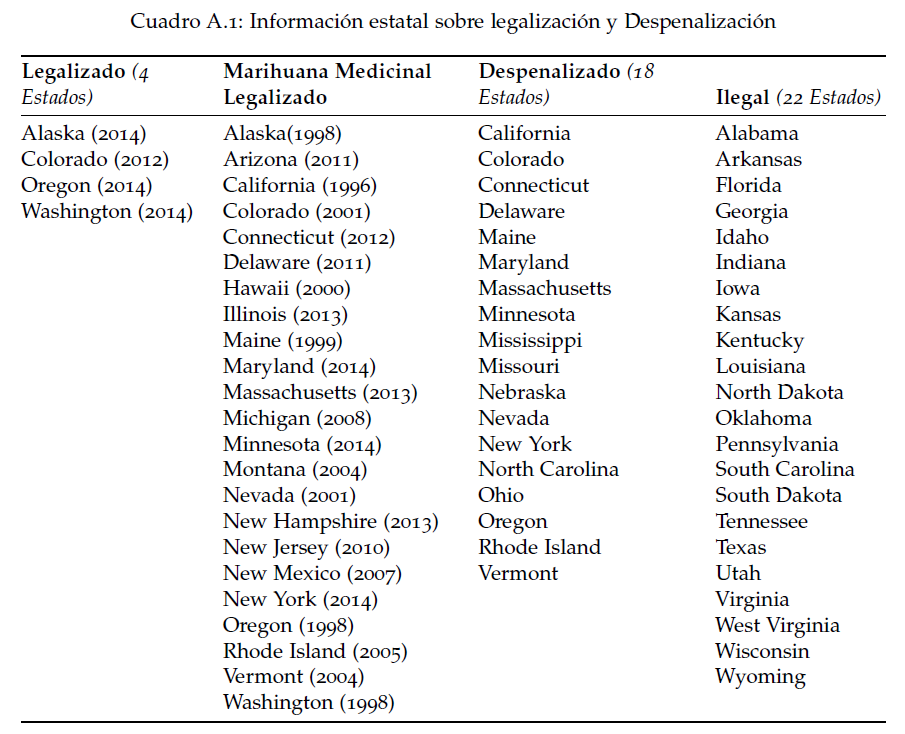
\includegraphics[width=0.82\textwidth,height=\textheight]{C:/Users/Usuario/Documents/Doc_espan/tb1.png}

\end{frame}

\hypertarget{metodos}{%
\section{Métodos}\label{metodos}}

\begin{frame}{Datos y medidas}
\protect\hypertarget{datos-y-medidas}{}

\begin{block}{Variable Dependiente}

(Asesinato y homicidio no negligente, Violación, Robo y Asalto agravado)
entre 1980 y 2014 se obtuvieron del \emph{FBI's Uniform Crime Reporting}
\href{https://bjs.gov/}{(UCR)}

\end{block}

\begin{block}{Variable Independiente}

El año de inicio de la LM se obtuvo del sitio web oficial
\href{https://norml.org/states}{NORML}. La variable de Dummy representa
el número de años que la ley ha estado vigente

\end{block}

\begin{block}{Variables de Control}

\begin{itemize}
\tightlist
\item
  El porcentaje de la fuerza laboral civil desempleada de cada estado,
  se obtuvo del sitio web de la Oficina de Estadísticas Laborales
  (\href{https://www.bls.gov/lau/}{BLS})
\item
  La tasa de empleo total, se obtuvo del sitio web de la Oficina de
  Estadísticas Laborales (\href{https://www.bls.gov/sae/}{BLS})
\item
  El porcentaje de la población que vive por debajo del umbral de
  pobreza, se obtuvo de la
  \href{https://www.census.gov/topics/income-poverty/poverty.html}{Oficina
  del Censo}
\item
  La tasa de consumo de cerveza per cápita
\end{itemize}

\end{block}

\end{frame}

\begin{frame}{Plan de Análisis}
\protect\hypertarget{plan-de-analisis}{}

Un diseño de de panel de efectos aleatorios, para la LM en los 50
estados durante el período de observación de 22 años

\begin{table}[!htbp] \centering 
  \caption{Porcentaje de los datos faltantes antes de la imputación} 
  \label{tab:misst} 
\begin{tabular}{@{\extracolsep{5pt}} lc} 
\\[-1.8ex]\hline 
\hline \\[-1.8ex] 
\textbf{Variables} & \textbf{\% Faltantes} \\ 
\hline \\[-1.8ex] 
Homicidio & 0.00\% \\ 
Violación & 0.00\% \\ 
Robo & 0.00\% \\ 
Asalto Agravado & 0.00\% \\ 
Tasa de Pobreza & 38.38\% \\ 
Tasa de Empleo & 1.96\% \\ 
Tasa de Desempleo & 1.96\% \\ 
Galones de cerbeza per capita & 1.96\% \\ 
Post-Ley & 0.00\% \\ 
\hline \\[-1.8ex] 
\end{tabular} 
\end{table}

\end{frame}

\hypertarget{resultados}{%
\section{Resultados}\label{resultados}}

\hypertarget{resultados-preliminares}{%
\subsection{Resultados Preliminares}\label{resultados-preliminares}}

\begin{frame}{Resultados Preliminares}
\protect\hypertarget{resultados-preliminares-1}{}

\begin{block}{Tendencia (lado izquierdo)}

Criminalidad por año, para los estados que no aprobaron la LM. Por lo
tanto,

\end{block}

\begin{block}{Tendencia (lado derecho)}

Los estados que aprobaron la LM contribuyen la recta hasta el año hasta
el año vigente de aprobación de la LM.

\begin{figure}
\centering
\includegraphics[width=0.5\textwidth,height=\textheight]{C:/Users/Usuario/Documents/Doc_espan/pol_imp3.png}
\caption{Regresión Discontinua de la tasa de Criminalidad en función de
los años}
\end{figure}

\end{block}

\end{frame}

\begin{frame}{Resultados Preliminares}
\protect\hypertarget{resultados-preliminares-2}{}

La recta del lado derecho revela estos estados experimentaron una
reducción de crimen gradualmente para los estados de California y New
Jersey a comparación del segundo estado con mayor población Texas en
donde la LM es Ilegal.

Estos \textbf{RESULTADOS PRELIMINARES} sugieren que la LM puede tener un
efecto de reducción del crimen, pero hay que tomar en cuenta que otros
factores pueden estar relacionados con las tendencias de las series de
tiempo que no se han tomado en cuenta para estas regresiones. Cuadro A.4

\end{frame}

\begin{frame}{Regresión}
\protect\hypertarget{regresion}{}

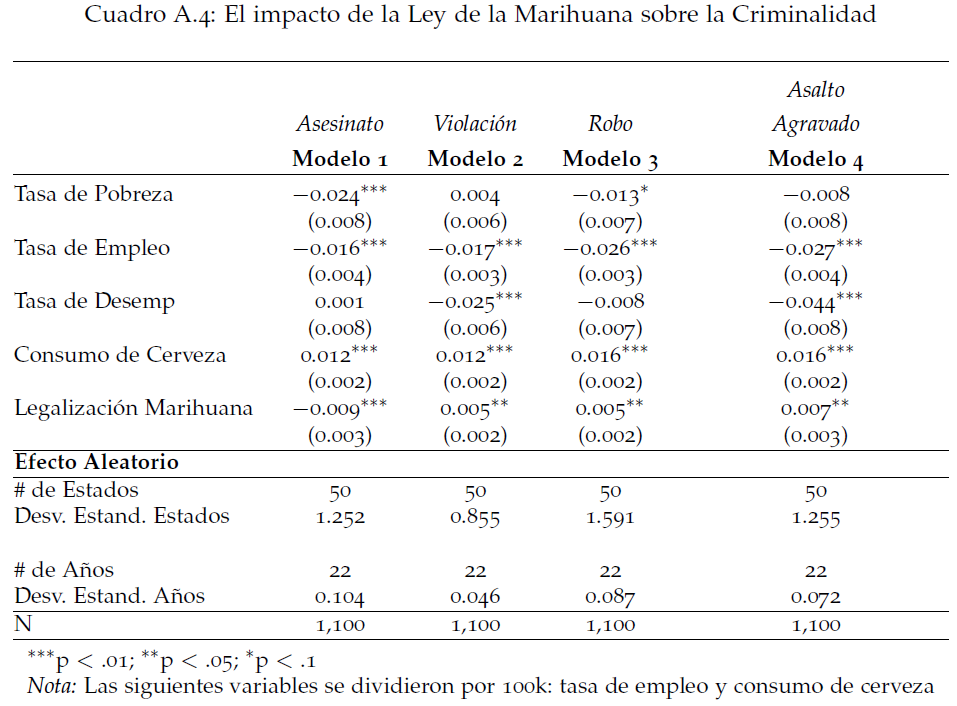
\includegraphics{C:/Users/Usuario/Documents/Doc_espan/tb4.png}

\end{frame}

\begin{frame}{Regresión}
\protect\hypertarget{regresion-1}{}

\includegraphics{Marh_svm_files/figure-beamer/graph3-1.pdf}

\end{frame}

\hypertarget{conclusiones}{%
\section{Conclusiones}\label{conclusiones}}

\begin{frame}{Conclusiones}
\protect\hypertarget{conclusiones-1}{}

\begin{itemize}
\tightlist
\item
  La investigación empírica sobre la relación entre las leyes sobre la
  Marihuana y el crimen son escasas y las consecuencias del consumo de
  marihuana en el crimen siguen siendo desconocidas. Por lo que al final
  \textbf{no se encontró que la LM tenga un efecto de mejora del crimen}
  para ninguno de los tipos de delitos analizados.
\item
  Los resultados se ajustan a la evidencia reciente y se ajustan a la
  idea de que la legalización de la marihuana puede llevar a una
  reducción en el consumo de alcohol
\item
  Los hallazgos actuales también deben tomarse en contexto con la
  naturaleza de los datos disponibles

  \begin{itemize}
  \tightlist
  \item
    No se tienen en cuenta los delitos que no se denunciarona la policía
  \item
    Al igual que la delincuencia juvenil
  \end{itemize}
\end{itemize}

\emph{La reproducción del escrito y láminas se encuentra en}
\textbf{github-com/cristian1512}

\end{frame}

\hypertarget{referencias}{%
\section{Referencias}\label{referencias}}

\begin{frame}{Referencias}
\protect\hypertarget{referencias-1}{}

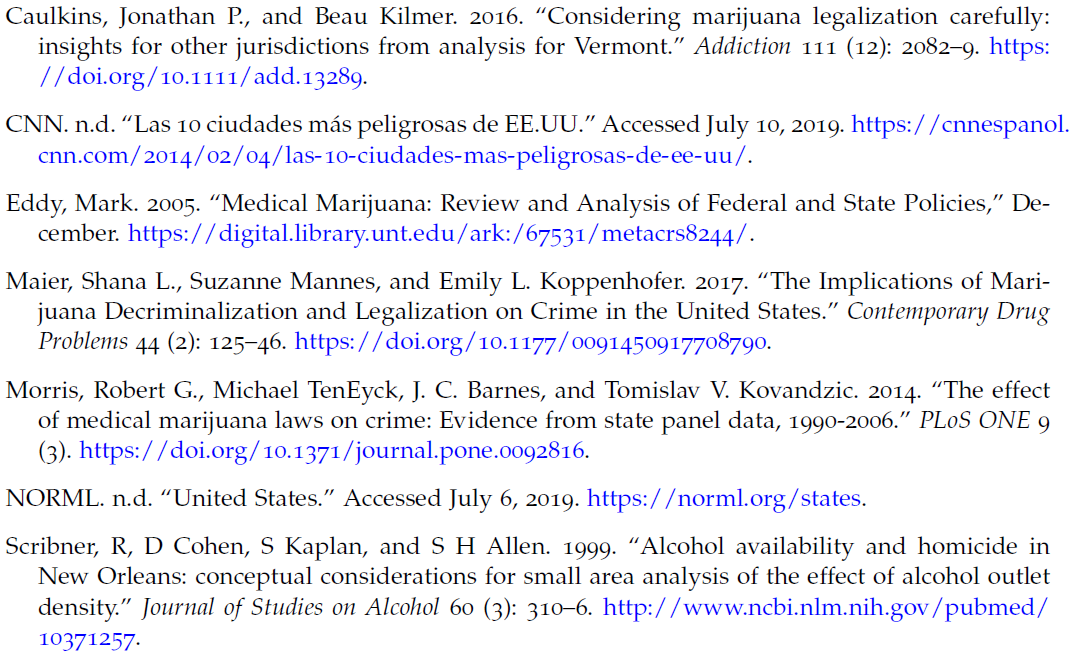
\includegraphics{C:/Users/Usuario/Documents/Doc_espan/ref.png}

\end{frame}


\section[]{}
\frame{\small \frametitle{Table of Contents}
\tableofcontents}
\end{document}
